\documentclass{article}
\usepackage{graphicx}
\usepackage{float}
\usepackage{subcaption}
\usepackage{amsmath}
\usepackage[colorlinks=true, allcolors=blue]{hyperref}
\bibliographystyle{unsrtnat}
\usepackage[square, numbers]{natbib}

\bibliographystyle{alpha}

\title{Information Theory \\ \large Problem Set 04 - Symbol Codes}
\author{Luís Felipe Ramos Ferreira}
\date{\href{mailto:lframos\_ferreira@outlook.com}{\texttt{lframos\_ferreira@outlook.com}}
}

\begin{document}

\maketitle

\begin{enumerate}
	\item \begin{enumerate}
		      \item A (binary) symbol code for an ensemble, denoted by \(C\), is a function that maps the outcomes of the ensemble to a set os binary strings. In particular, this set of strings is a subset of \(\{0, 1\}^+\), which denotes the set of all binary strings of non zero length. The extended code for the ensemble, denoted by \(C^+\), is a function from \(\mathcal{A}_X^+\) to \(\{0, 1\}^+\). More precisely, it represents the concatenation of the codewords of a ordered set of outcomes from the ensemble.
		      \item A symbol code is uniquely decodeable when no element is mapped to the same codeword. It is easy to see that is true based on the pidgeonhole principle. More formally, a code \(C(x)\) is uniquely decodeable if, under the extended code \(C^+\), we have:
		            \[\forall x, y \in \mathcal{A}_X^+, x \neq y \Rightarrow c^+(x) \neq c^+(y)\]
		            A symbol code is prefix-free if no codeword is a prefix of any other codeword, as stated by McKay \cite{MacKay}.
		      \item The Kraft inequality says that, for any uniquely decodeable code \(C(x)\) over the alphabet \(\{0,1\}\), the length \(l_i\) of the codewords must satisfy:
		            \[\sum_{i=1}^{I}2^{-l_i} \leq 1\],
		            where \(I = |\mathcal{A}_X|\).
		            Kraft and McMillan proved the intrinsic relation between de Kraft iunequality and prefix codes. In general, a set of codewords lengths satisfies the Kraft inequality if and only if there exists a prefix code with the given lengths. So they are two complete tied concepts.
		      \item The source coding theorem for symbol codes states that for a ensemble \(X\), there is a prefix code \(C\) whose expected length \(L(C, X)\) satisfies the following inequality:
		            \[H(X) \leq L(C, X) \leq H(X) + 1\],
		            where \(H(X)\) denotes the entropy of the ensemble \(X\).
		            So, at a high level, the optimal prefix code for the ensemble has a expected length very close to the entropy of the ensemble. Such a prefix code is the best way to compress the outcomes of the ensemble \(X\) in a binary encoding, i. e. the entropy of the ensemble is the limit for the amount of bits per symbol of a prefix free encoding. Also, one can always use a prefix free encoding and achieve a result with at most \(H(X) + 1\) bits per symbol.
	      \end{enumerate}

	\item No, it is not uniquely decodeable, since there are codewords that are prefixer of others. The string 111111, for example, could represent three uses of the code 111 or two uses of the code 111.
	\item Yes, it is, since it is prefix free.
	\item Handmade exercise.
	      \begin{enumerate}
		      \item First part
		            \begin{figure}[H]
			            \centering
			            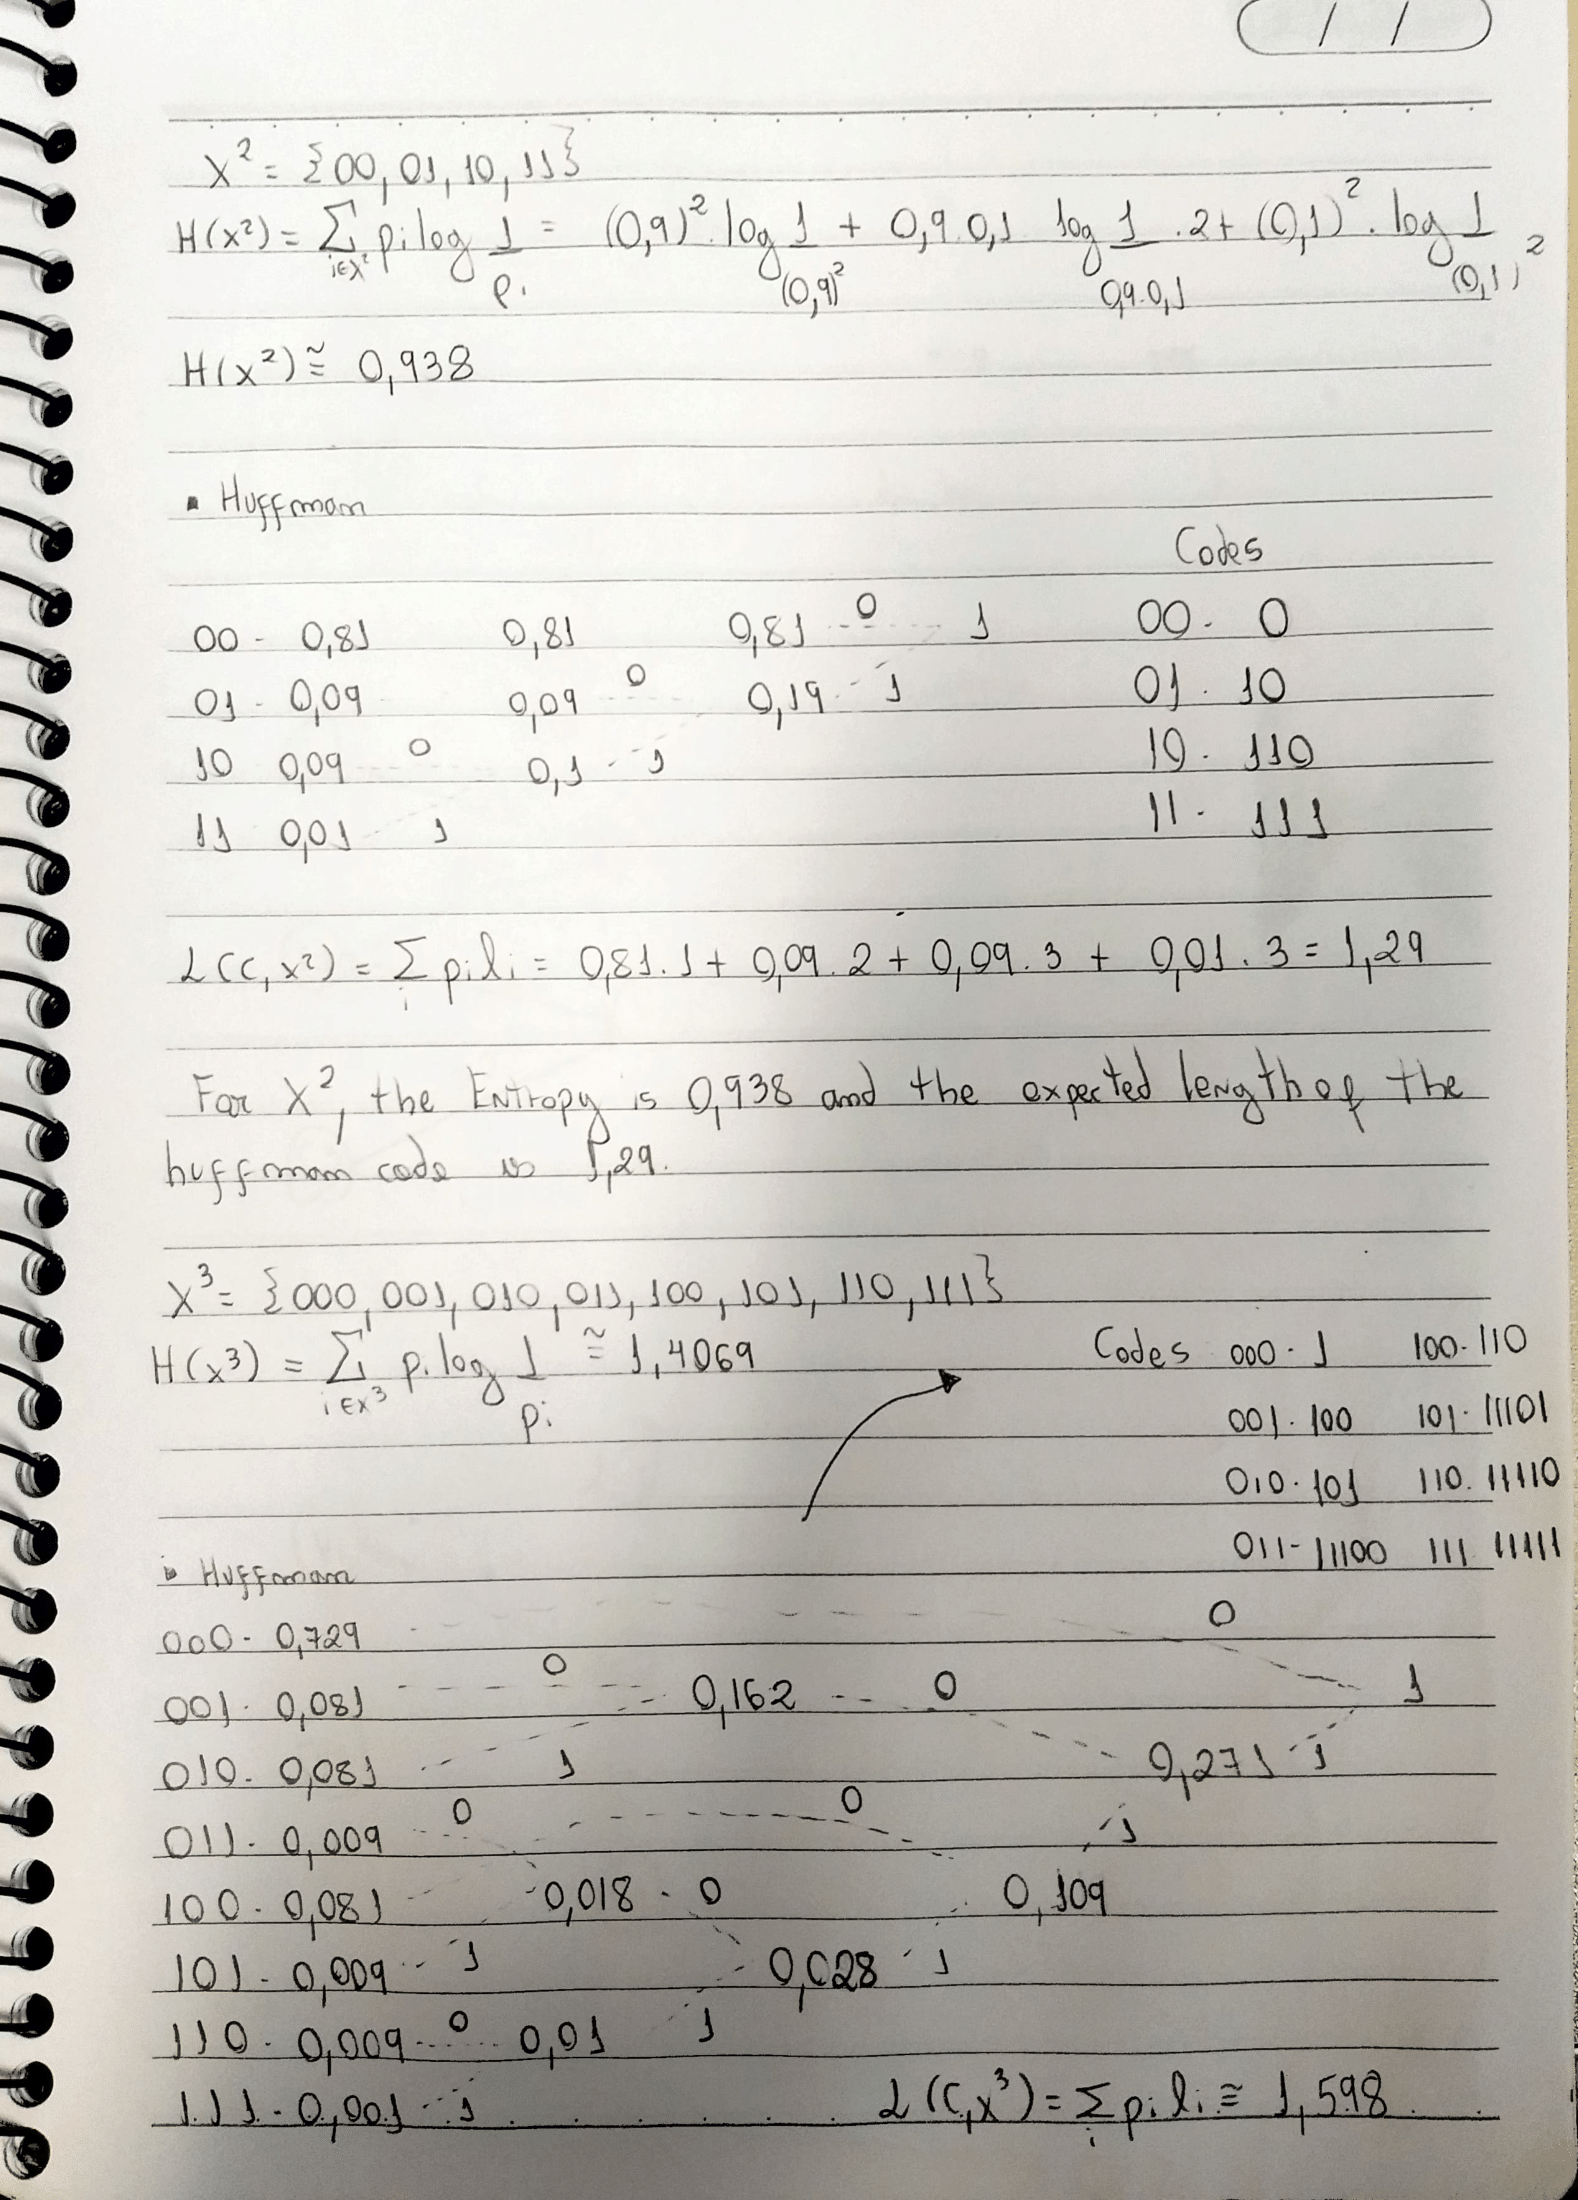
\includegraphics[width=0.8\textwidth]{images/it1-1.png}
		            \end{figure}
		      \item Second part
		            \begin{figure}[H]
			            \centering
			            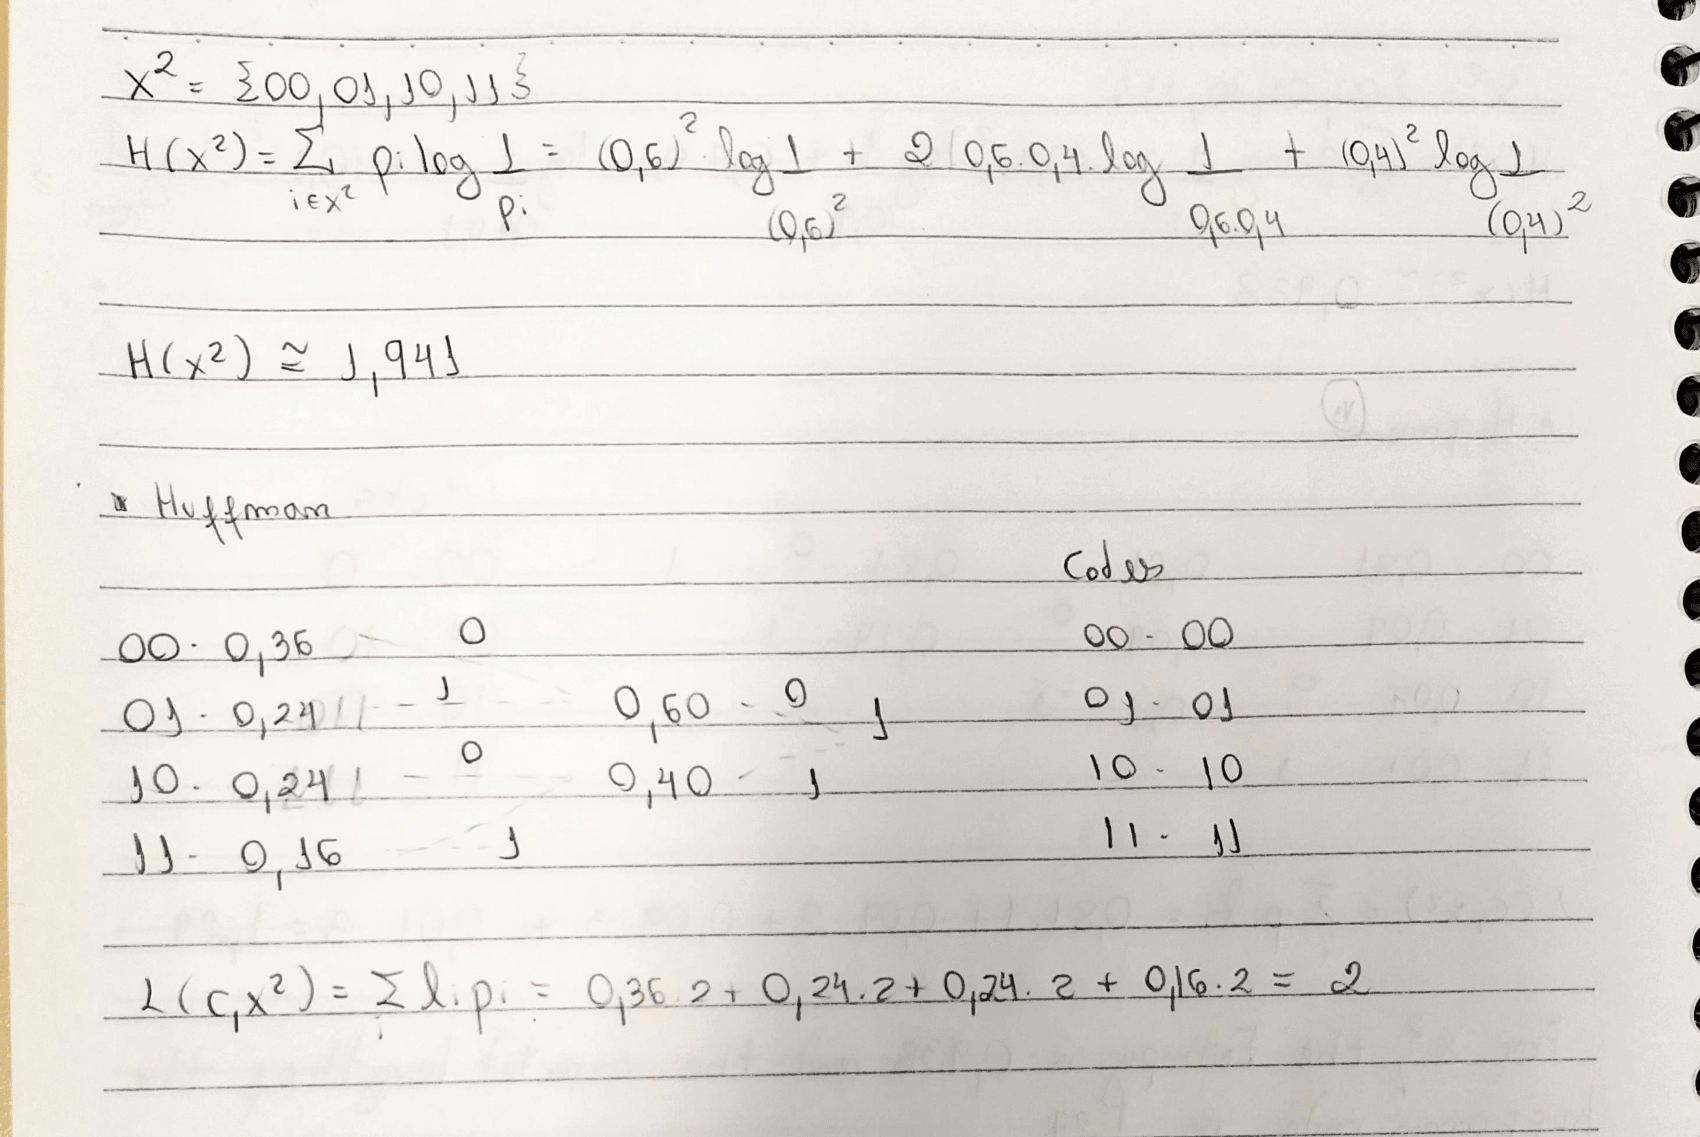
\includegraphics[width=0.8\textwidth]{images/it2-1.png}
		            \end{figure}
	      \end{enumerate}
	\item We know that Huffman codes are optimal for symbol codes. We will show that the following probability distribution \(S\) give \textit{two} different optimal codes that assing different lengths to the symbols.
	      \[S = \{1/6,1/6,1/3,1/3\}\]
	      \begin{figure}[H]
		      \centering
		      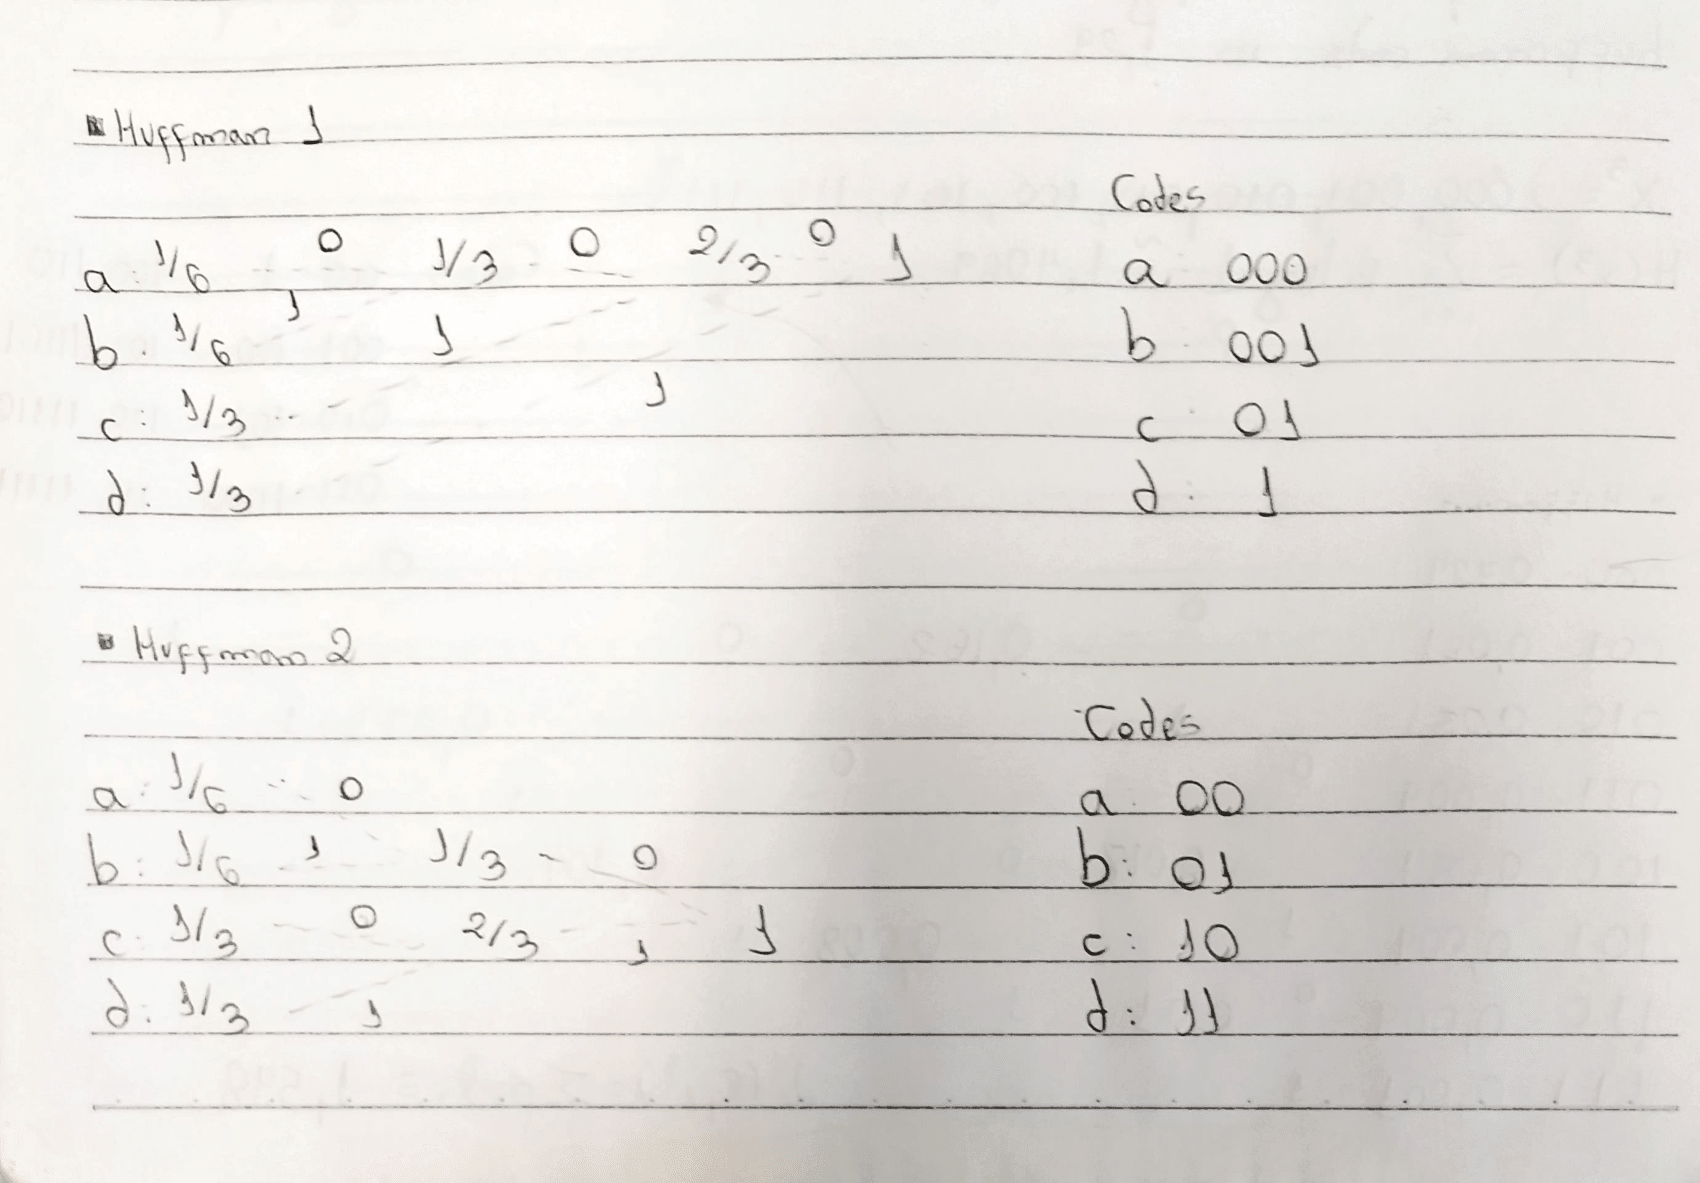
\includegraphics[width=0.8\textwidth]{images/it3-1.png}
	      \end{figure}

	      This happens because in the second step there is more than one option to choose to create de Huffman encoding.

	\item To play the \textbf{twenty questions} optimally, it is necessary to find a set of binary questions that guarantees you to eliminate half or as close as possible to half of the current options for the answer. This ensures the number of questions to be asked to be always of the order of \(log N\), where \(N\) is the number of elements in the universe. To find such set of questions, several approaches can be made, given the properties of the elements of the universe. One of them is to find some kind of order in the set of elements of the universe. With such an ordering, one can apply a binary search algorithm to find the desired object.

	      But why is this the optimal startegy? Because it ENSURES the correct guess will be made in an order of \(N\) of the number of possible objects in the universe. Supose you ask a specific question like: "is the object A?". You could be lucky and get it right on the first try, but the probability of this happening is very low. Particularly, the largest \(N\) is, the lower the probability you would win on the first 20 rounds of questions. With the previous mentioned approach, luck doesn't matter, you will ALWAYS get to the answer in an order of \(log N\) questions, and that's why it is the optimal solution to the game.

\end{enumerate}

\bibliography{sample}

\end{document}
